%%%%%%%%%%%%%%%%%%%%%%%%%%%%%%%%%%%%%%%%%%%%%%

\begin{frame}
    \frametitle{Operaciones sobre la variable independiente I}
    \begin{itemize}
        \item Transformación $f(t)$ en la variable independiente:\\
        \vspace{0.1cm}
        \begin{center}
            \color{blue}$x(t)\Rightarrow y(t) = x(f(t))$, \hspace{0.1cm} $x[n] \Rightarrow y[n]=x[f(n)]$\color{black}
        \end{center}
        \vspace{0.1cm}
        \item Aunque no alteran los valores de la señal, pueden... 
        \vspace{0.2cm}
        \begin{itemize}
            \item alterar la forma
            \item provocar la pérdida de muestras (caso discreto).
        \end{itemize}
        \vspace{0.2cm}
        \item Suponemos\footnote{Veremos otras transformaciones en el Tema 5} \color{blue}$f(t)=\alpha t+\beta$\color{black}
        \vspace{0.4cm}

        \begingroup
            \small
            \begin{tabular}{r|ll}
                & continuo & discreto\\\hline
                \color{red}Desplazamiento:\color{black} & $y(t)=x(t-t_0)$ & $y[n]=x[n-n_0]$ \\
                \color{red}Inversión:\color{black} & $y(t)=x(-t)$ & $y[n]=x[-n]$ \\
                \color{red}Compresión/Expansión:\color{black} & $y(t)=x(\alpha t)$ & $y[n]=x[Kn]$ \\
            \end{tabular}
        \endgroup
    \end{itemize}
\end{frame}

%%%%%%%%%%%%%%%%%%%%%%%%%%%%%%%%%%%%%%%%%%%%%%

\begin{frame}
  \frametitle{Operaciones sobre la variable independiente II}
  \vspace{-0.1cm}
  \begin{itemize}
    \item <1-> \alert{Desplazamiento temporal:}
    \begin{itemize}
      \vspace{0.1cm}
      \item Continuo: $x(t) \: \rightarrow y(t)=x(t-t_0)$
      \vspace{0.1cm}
      \item Discreto: $x[n] \: \rightarrow y[n]=x[n-N_0]$
    \end{itemize}
    \vspace{0.2cm}
    \item <1-> \alert{Inversión:}
    \begin{itemize}
      \vspace{0.1cm}
      \item Continuo: $x(t) \: \rightarrow y(t)=x(-t)$
      \vspace{0.1cm}
      \item Discreto: $x[n] \: \rightarrow y[n]=x[-n]$
    \end{itemize}
  \end{itemize}
  \vspace{-0.3cm}
  \begin{figure}
    \centering
    \footnotesize
    \begin{tabular}{@{\extracolsep{-8pt}}cc}
      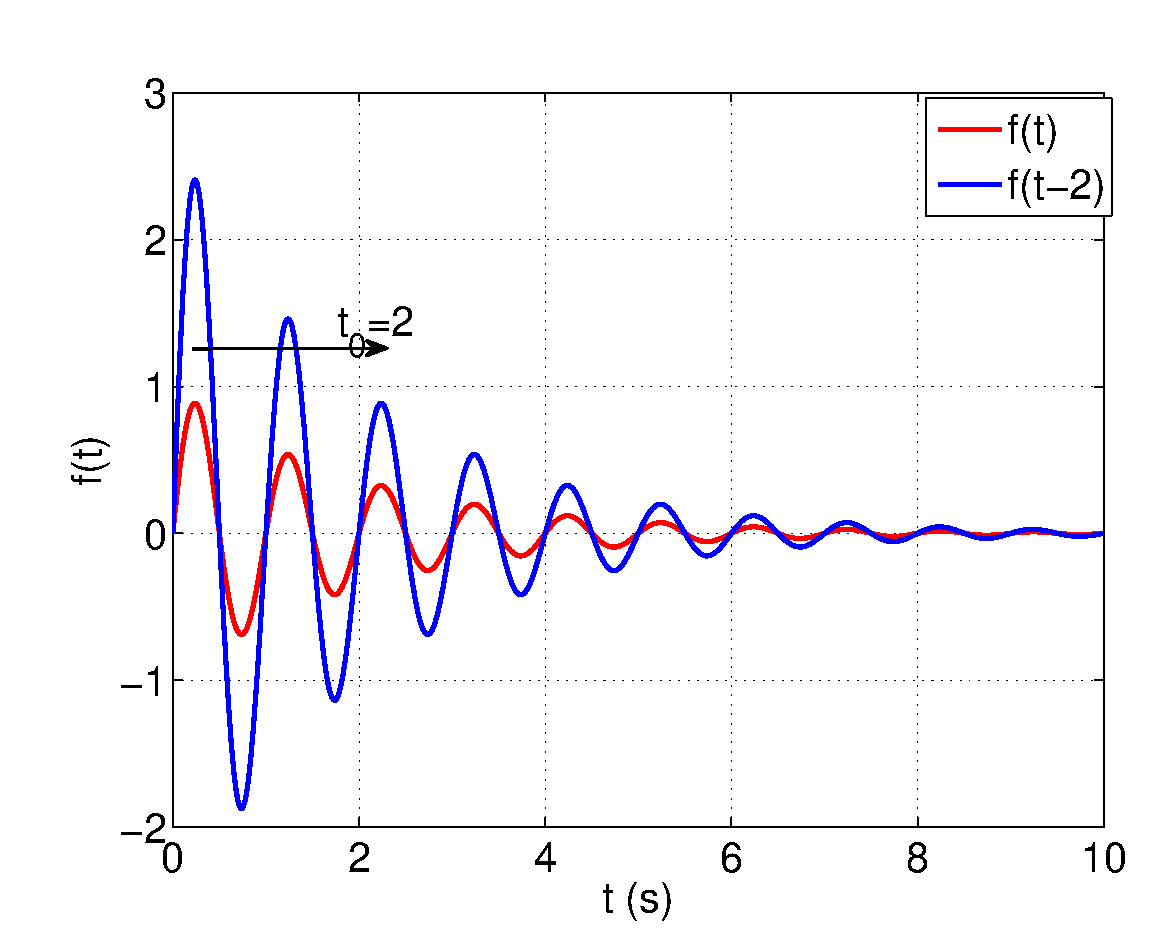
\includegraphics[width=4.5cm]{./Figuras/Figures/DesplazamientoT.eps}&
      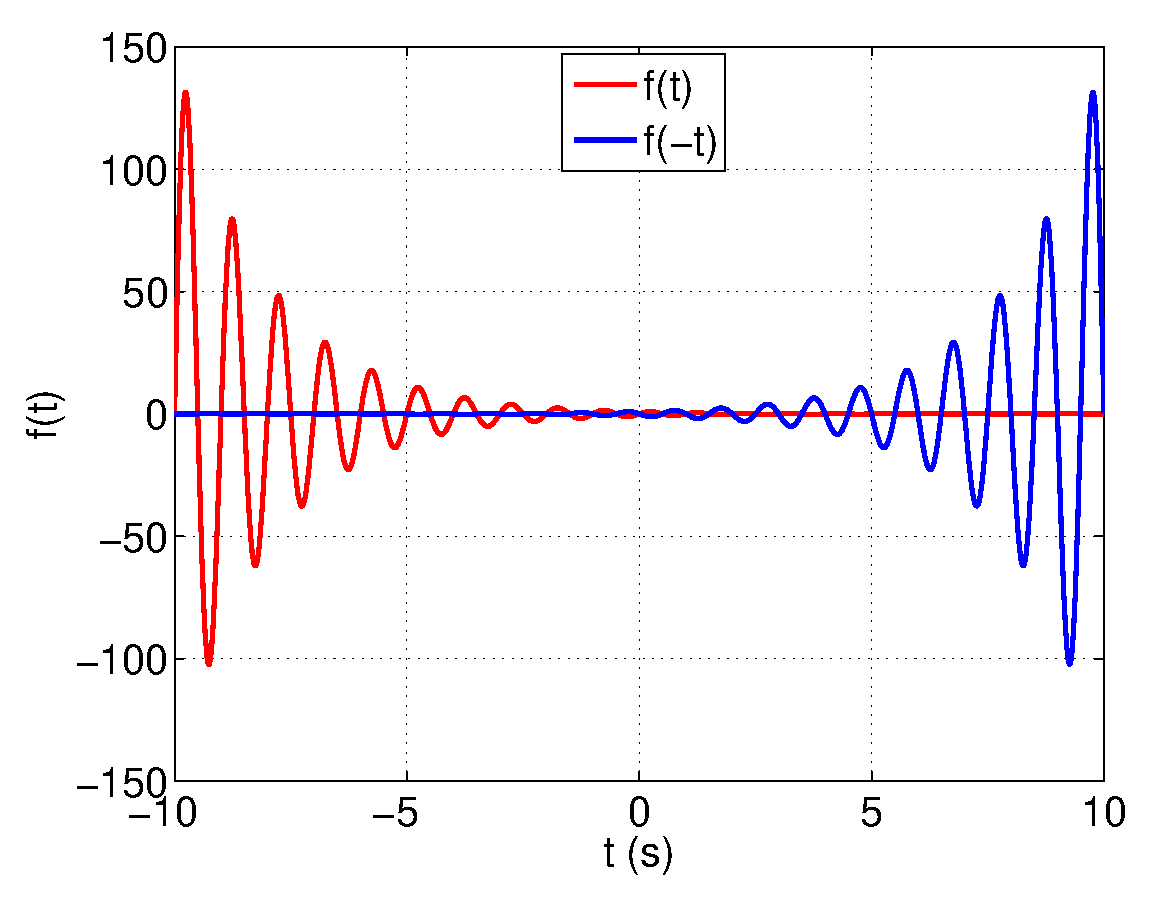
\includegraphics[width=4.5cm]{./Figuras/Figures/Inversion.eps} \\
      Desplazamiento  & Inversión
    \end{tabular}
  \end{figure}
\end{frame}

%%%%%%%%%%%%%%%%%%%%%%%%%%%%%%%%%%%%%%%%%%%%%%

\begin{frame}
  \frametitle{Operaciones sobre la variable independiente III}
  \vspace{-0.1cm}
  \begin{itemize}
    \item <1-> \alert{Compresión/expansión temporal}:
    \begin{itemize}
      \vspace{0.1cm}
      \item Continuo (escalado): \color{blue}$x(t) \: \rightarrow y(t)=x(\alpha \cdot t), \alpha>0$\color{black}
      \begin{itemize}
        \item Compresión ($\alpha > 1$), Expansión ($\alpha < 1$) 
      \end{itemize}
      \vspace{0.1cm}
      \item Discreto:
      \vspace{0.1cm}
      \begin{itemize}
        \item Diezmado:  \color{blue}$x[n] \: \rightarrow y[n]=x[N\cdot n], N \in \mathbb{Z}^+$\color{black}
        \vspace{0.1cm}
        \item Interpolación: \color{blue}$x[n] \: \rightarrow y[n]=x[\frac{n}{N}], N \in \mathbb{Z}^+$\color{black} \\
            \color{cyan}{\scriptsize no existe muestra para $\frac{n}{N}$ no entero, necesario generar}\color{black}
      \end{itemize}
    \end{itemize}
  \end{itemize}
  \vspace{-0.3cm}
  \begin{figure}
    \centering
    \footnotesize
    \begin{tabular}{@{\extracolsep{-8pt}}cc}
      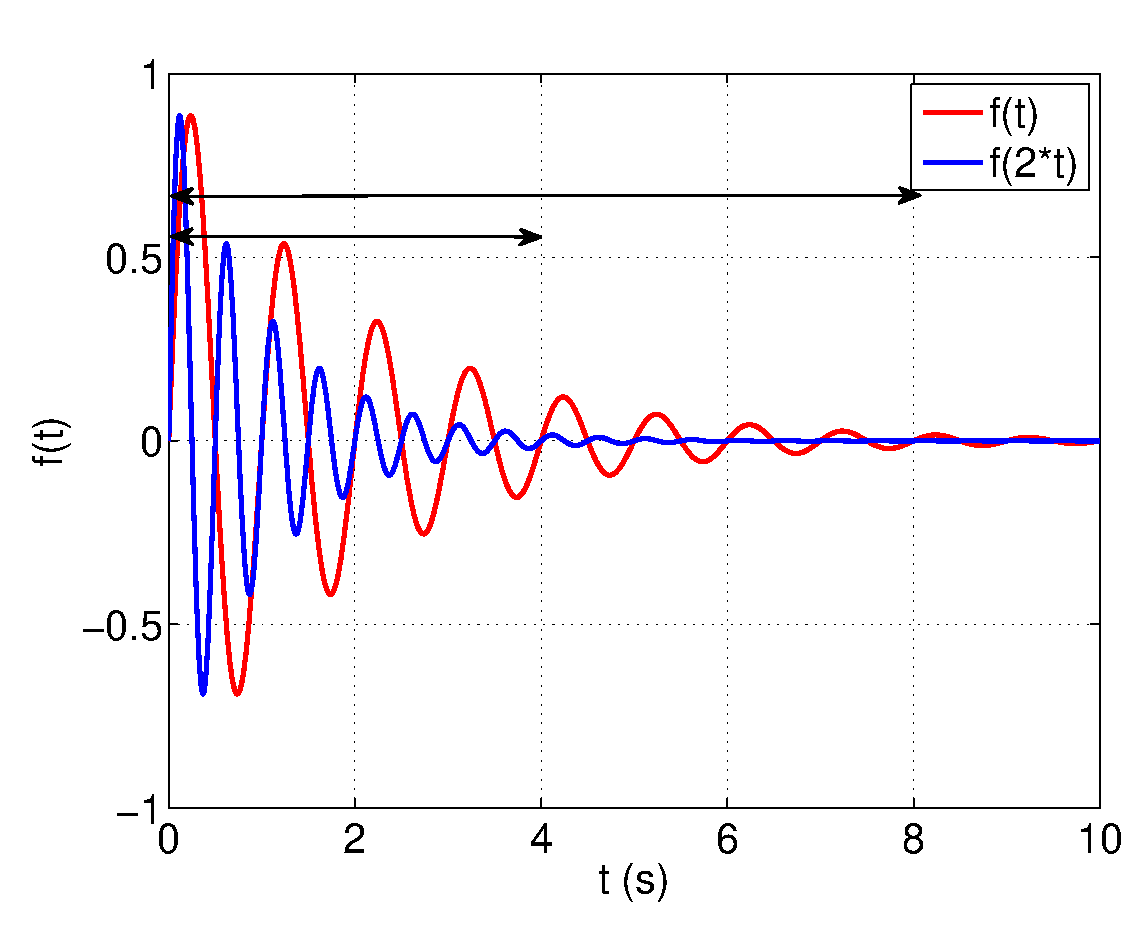
\includegraphics[width=4.5cm]{./Figuras/Figures/EscaladoT.eps}&
      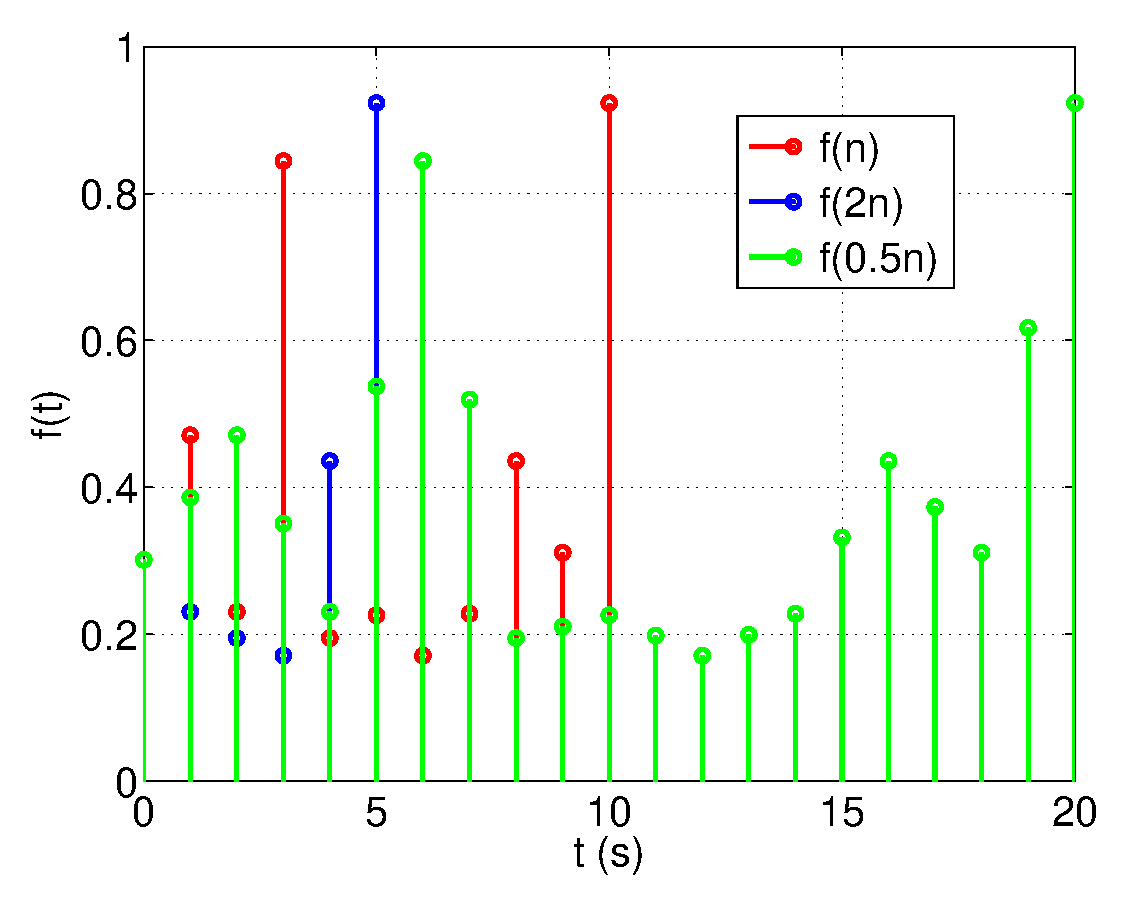
\includegraphics[width=4.4cm]{./Figuras/Figures/EscaladoD.eps} \\
      Escalado & Diezmado \& Interpolación
    \end{tabular}
  \end{figure}
\end{frame}

% %%%%%%%%%%%%%%%%%%%%%%%%%%%%%%%%%%%%%%%%%%%%%%%%%%%

\begin{frame}
  \frametitle{Operaciones básicas sobre la señal}
  \begin{itemize}
    \item \color{red}Generales\color{black}:
    \begin{itemize}
      \vspace{0.1cm}
      \item  {Suma/Resta/Multiplicación/División}:\\
      \vspace{0.1cm}
      \color{blue}$x_1(\cdot) \pm x_2(\cdot)$,   $\:\:x_1(\cdot) \cdot x_2(\cdot)$,  $\:\:x_1(\cdot) \div x_2(\cdot)$\color{black}
    \end{itemize}
    \vspace{0.1cm}
    \item{\color{red}Continuas\color{black}}:
    \begin{itemize}
      \vspace{0.1cm}
      \item Derivación: \color{blue}$y(t)=\frac{dx(t)}{dt}$\color{black}
      \vspace{0.2cm}
      \item Integración: \color{blue}$y(t)=\int_{\tau=-\infty}^t x(\tau) d\tau$\color{black}
      \vspace{0.1cm}
    \end{itemize}
    \item{\color{red}Discretas\color{black}}:
    \begin{itemize}
      \vspace{0.1cm}
      \item Diferencia: \color{blue}$y[n]=x[n]-x[n-1]$\color{black}
      \vspace{0.2cm}
      \item Acumulación: \color{blue}$x[n]=\sum_{k=-\infty}^n x[k]$\color{blue}
      \vspace{0.1cm}
    \end{itemize}
  \end{itemize}
\end{frame}

% %%%%%%%%%%%%%%%%%%%%%%%%%%%%%%%%%%%%%%%%%%%%%%%%%%%

\begin{frame}
  \frametitle{Convolución}
  \begin{itemize}
    \item Convolución de dos señales:
    \vspace{0.1cm}
    \begin{itemize}
      \item \alert{Señales continuas}: \small \color{blue}$(x \ast y)(t)=\int_{-\infty}^\infty x(\tau)y(t-\tau)d\tau$\color{black}
      \vspace{0.1cm}
      \item \alert{Señales discretas}: \small \color{blue}$(x \ast y)[n]=\sum_{k=-\infty}^\infty x[k]y[n-k]$\color{black}
      \begin{itemize}
        \vspace{0.2cm}
        \item Invertir:\quad\quad \color{cyan}$y(-\tau), y[-k].$\color{black}
        \item Desplazar:~~ \color{cyan}$y(t-\tau), y[n-k].$\color{black}
        \item Multiplicar:~~ \color{cyan}$x(\tau)y(t-\tau), x[k]y(n-k).$\color{black}
        \item Sumar:\quad\quad \color{cyan}$\int, \sum.$\color{black}
      \end{itemize}
    \end{itemize}
    \vspace{0.2cm}
    \item Propiedades:
    \begin{itemize}
      \small
      \item Conmutativa:  $(x \ast y)(\cdot)=(y\ast x)(\cdot)$
      \item Asociativa: $(x \ast y \ast z)(\cdot)=[(x \ast y) \ast z](\cdot)=[x \ast( y \ast z)](\cdot)$
      \item Distributiva: $((x+y) \ast z)(\cdot)=(x \ast z)(\cdot)+(y \ast z)(\cdot)$
      \item Respecto al impulso y al escalón  (más adelante)
    \end{itemize}
  \end{itemize}
\end{frame}


\begin{frame}\frametitle{Fourier (Cuadro resumen)}
  
  \centering
  \begin{tabular}{>{\columncolor{lightgray}}ccc}
    \rowcolor{lightgray}
    & \color{blue}\small \alert{Continua}  & \color{blue}\small  \alert{Discreta}\\
    \rotatebox{90}{\color{red}\small Periódica\color{black}}    & \parbox{4cm}{\centering\tiny Series de Fourier Continuas (CFS)\\\color{blue}$c[k]=\frac{1}{T}\int_{-T/2}^{T/2}{x(t)e^{-j k\omega_0 t}dt}$\color{black}\\\color{blue}$x(t)=\sum_{k=-\infty}^{\infty}{c[k]e^{j k\omega_0 t}}$\color{black}} & \parbox{3.5cm}{\centering\tiny Series de Fourier Discretas (DFS)\\\color{blue}$c[k]=\frac{1}{N}\sum_{n=0}^{N-1}{x[n]e^{-j\frac{2\pi}{N} k n}}$\color{black}\\\color{blue}$x[n]=\sum_{k=0}^{N-1}{c[k]e^{j\frac{2\pi}{N} k n}}$\color{black}} \\\\
    \rotatebox{90}{\color{red}\small Aperiódica\color{black}}   & \parbox{4cm}{\centering\tiny Trasnformada de Fourier\\de Tiempo Continuo (CTFT)\\\color{blue}$X(j\omega)= \int_{-\infty}^{\infty} x(t) e^{j\omega t} dt $\color{black}\\\color{blue}$x(t)=\frac{1}{2\pi}\int_{-\infty}^{\infty}{X(j\omega)e^{j\omega t}d\omega}$\color{black}} & \parbox{4cm}{\centering\tiny Trasnformada de Fourier\\de Tiempo Discreto (DTFT)\\\color{blue}$X(e^{j\omega})=\sum_{k=-\infty}^{\infty}{x[n]e^{-j\omega n}}$\color{black}\\\vspace{0.1cm}\color{blue}$x[n]=\frac{1}{2\pi}\int_{0}^{2\pi}{X(e^{j\omega})e^{j\omega n}d\omega}$\color{black}} \\
  \end{tabular}
  \begin{flushleft}
    \small
    \begin{itemize}
      \item Transformada de Fourier Discreta (DFT):
      \begin{itemize}
        \item \color{blue}$X[k]=\sum_{n=0}^{N-1}{x[n]e^{-j\frac{2\pi}{N} k n}}$\color{black}\\\vspace{0.1cm}
        \item \color{blue}$x[n]=\frac{1}{N}\sum_{k=0}^{N-1}{X[k]e^{j\frac{2\pi}{N} k n}}$\color{black}
      \end{itemize}
  \end{itemize}
  \end{flushleft}
\end{frame}


\begin{frame}
  \frametitle{Desarrollo en serie de Fourier: Se\~{n}ales peri\'{o}dicas}
  \vspace{-0.1cm}
  \small
  \begin{itemize}
    \item \color{red}Señales continuas\color{black}:  \color{blue}$x(t)=x(t+T)$, $\omega_0=2\pi/T$\color{black}
    \begin{itemize}
      \footnotesize
      \item Desarrollo en exponenciales complejas:\\
      \vspace{0.1cm}
      $\color{blue}\bullet\color{black}$ S\'{i}ntesis: \color{blue}$x(t)=\sum_{k=-\infty}^\infty c_k e^{jk\omega_0t}$\color{black}\\
      $\color{blue}\bullet\color{black}$  Análisis:  \color{blue}$c_k=\frac{1}{T } \int_{T} x(t) e^{-jk\omega_0t} dt $\color{black}
      \vspace{0.1cm}
      \visible<2->{
      \item Desarrollo en senos y cosenos ($x(t)$ es real):\\
      \vspace{0.1cm}
      $\color{blue}\bullet\color{black}$ S\'{i}ntesis:  $x(t)=\frac{a_0}{2}+\sum_{k=1}^{\infty} \left (a_k cos(k\omega_0t) + b_k sin(k\omega_0t)\right )$\\
      $\color{blue}\bullet\color{black}$  Análisis:  $ a_k=\frac{2}{T}\!\int_T x(t) cos(k\omega_0t)dt, \: \: b_k=\frac{2}{T}\!\int_T x(t) sin(k\omega_0t)dt$}
      \vspace{0.1cm}
    \end{itemize}
    \item \alert{Señales discretas}:  \color{blue}$x[n]=x[n+N]$, $\omega_0=2\pi/N$\color{black}
    \begin{itemize}
      \footnotesize
      \visible<3->{
      \item Desarrollo en exponenciales complejas:\\
      \vspace{0.1cm}
      $\color{blue}\bullet\color{black}$ S\'{i}ntesis: \color{blue}$x[n]=\sum_{k=0}^{N-1} c_k e^{j\omega_0kn}$\color{black}\\
      $\color{blue}\bullet\color{black}$ Análisis:  \color{blue}$c_k=\frac{1}{N } \sum_{n=0}^{N-1} x[n] e^{-j\omega_0kn} $\color{black}, $c_k=c_{k+N}$}
      \vspace{0.1cm}
      \visible<4->{
      \item Desarrollo en senos y cosenos ($x[t]$ es real):\\
      \vspace{0.1cm}
      $\color{blue}\bullet\color{black}$ $L=\frac{N}{2}\qquad \quad$ o $\quad L=\frac{N-1}{2}$\\
      $\color{blue}\bullet\color{black}$ $LIM=L-1\;$ o $\quad K=L$\\
      $\color{blue}\bullet\color{black}$ S\'{i}ntesis:  $x(n)=\frac{a_0}{2}+\sum_{k=1}^{LIM} \left (a_k cos(k\omega_0kt) + b_k sin(\omega_0kt)\right )$\\
      $\color{blue}\bullet\color{black}$  Análisis:  ${ a_k=\frac{2}{N}\sum_{n=0}^{N-1} x(n) cos(\omega kn), \: \: b_k=\frac{2}{N}\!\sum_{n=0}^{N-1} x(n) sin(\omega kn)}$}
      \vspace{0.1cm}
    \end{itemize}
  \end{itemize}
\end{frame}

%%%%%%%%%%%%%%%%%%%%%%
\begin{frame}
  \frametitle{Transformadas}
  % \vspace{-0.2cm}
  \begin{itemize}
    \item \alert{Serie vs. Transformada}
    \begin{itemize}
      \item \alert{Si una señal es periódica}
      \begin{itemize}
        \item Representación mediante exp. armónicas: $\phi_k(t)=\mathrm{e}^{\:jk \omega_0 t}$. 
        \item Combinación lineal: $x(t)=\sum_{k=-\infty}^{\infty}a_k\phi_k(t)$.
      \end{itemize}
      \item \alert{Si una señal es aperiódica:}
      \begin{itemize}
        \footnotesize
        \item El sumatorio pasa a ser una integral: $\int_{\omega=-\infty}^{\infty}X(\omega)\phi(\omega)d\omega$.
        \vspace{0.1cm}
      \end{itemize}
    \end{itemize}
    \item \alert{Transformada de Fourier, Laplace y Z:}
    \begin{itemize}
      \footnotesize
      \vspace{0.1cm}
      \item \alert{Se\~{n}ales continuas $x(t)$}:
      \begin{itemize}
        \footnotesize
        \item Transformada de Fourier: \color{blue}$X(j\omega_c)= \int_{-\infty}^{\infty} x(t) e^{-j\omega_c t} dt $\color{black}
        \item Transformada de Laplace: \color{blue}$X(s)=\int_{0}^{\infty} x(t) e^{-st} dt$\color{black}
        \item $s=\sigma \pm j\omega$
      \end{itemize}
      \visible<2->{
      \item \alert{Se\~{n}ales discretas $x[n]$}:
      \footnotesize
      \begin{itemize}
        \footnotesize
        \item T. de Fourier en tiempo discreto: \color{blue}$X(e^{j\omega_d})= \sum_{n=-\infty}^{\infty} x[n] e^{-j\omega_dn} $\color{black}
        \item Transformada Z: \color{blue}$X(z)=\sum_{n=0}^{\infty} x[n] z^{-n}$\color{black}
        \item  $X(e^{j\omega_d})$ es periodica (se repite en frecuencias cada $2\pi$)
        \item $z=e^{j\omega_d}$
        \item Si muestreamos periodicamente: $t=nT$, $z=e^{sT}$
      \end{itemize}
    }\end{itemize}
  \end{itemize}
\end{frame}

%%%%%%%%%%%%%%%%%%%%%%
\begin{frame}
  \frametitle{Transformadas}
  \vspace{-0.3cm}
  \begin{itemize}
    \item \alert{Comparación entre transformadas y sus usos:}
    \begin{itemize}
      \footnotesize
      \visible<3->{
      \item Transformada de Laplace y Z permiten:
      \begin{itemize}
        \scriptsize
        \item Resolver ecuaciones diferenciales (en diferencias)
        \item Obtener la funci\'{o}n de transferencia de sistemas LTI y su respuesta temporal a trav\'{e}s de la transformada inversa del producto de la funci\'{o}n de transferencia y la transformada de la entrada.
        \item Ver la respuesta a las condiciones iniciales.
      \end{itemize}
      }
      \visible<4->{
      \item Fourier (CTFT y DTFT) permite:
      \footnotesize
      \begin{itemize}
        \scriptsize
        \item Estudiar el comportamiento en frecuencia de las se\~{n}ales y de los sistemas.
        \item  Obtener la repuesta permanente de sistemas LTI estables como la transformada inversa del producto de la transformada de Fourier del sistema  con la transformada de la entrada.
      \end{itemize}
      }
    \end{itemize}
  \end{itemize}
\end{frame}


\begin{frame}\frametitle{Conceptos importantes}
  \begin{itemize}
    \item \alert{Operaciones sobre la variable independiente}
    \begin{itemize}
      \item Desplazamiento
      \item Inversión
      \item Compresión/Expansión
    \end{itemize}
    \item \alert{Operaciones básicas.}
    \begin{itemize}
      \item Generales (suma, resta, multiplicación, división)
      \item Derivación / Diferencia
      \item Integración / Acumulación
    \end{itemize}
    \item \alert{Convolución}
    \item \alert{Fourier}
  \end{itemize}
\end{frame}